%!TEX root = ../Manuale.tex
%%--------------------------------------------------------------------------
%% DISPOSITIVI
%%--------------------------------------------------------------------------



\chapter{Devices}
The section dedicate to the list of devices uses the concept of ``card'' means any device is displayed along with the details within a ``card''. On a smartphone the list will be in single column, on a device with a larger screen size will increase the number of columns. Each ``card'' shows the number of active alarms on the device, its color, the last date on which it was seen, and the group to which it belongs. Through a special item in the menu you can view the device on a map. \\ 
In this screen you can also view the list of devices filtered according to certain parameters; to do this there is a button on the ActionBar which will open a dialog box where you can choose the criteria and confirm.



	\begin{figure}[h!]
		  \centering
		    \centering{%
		      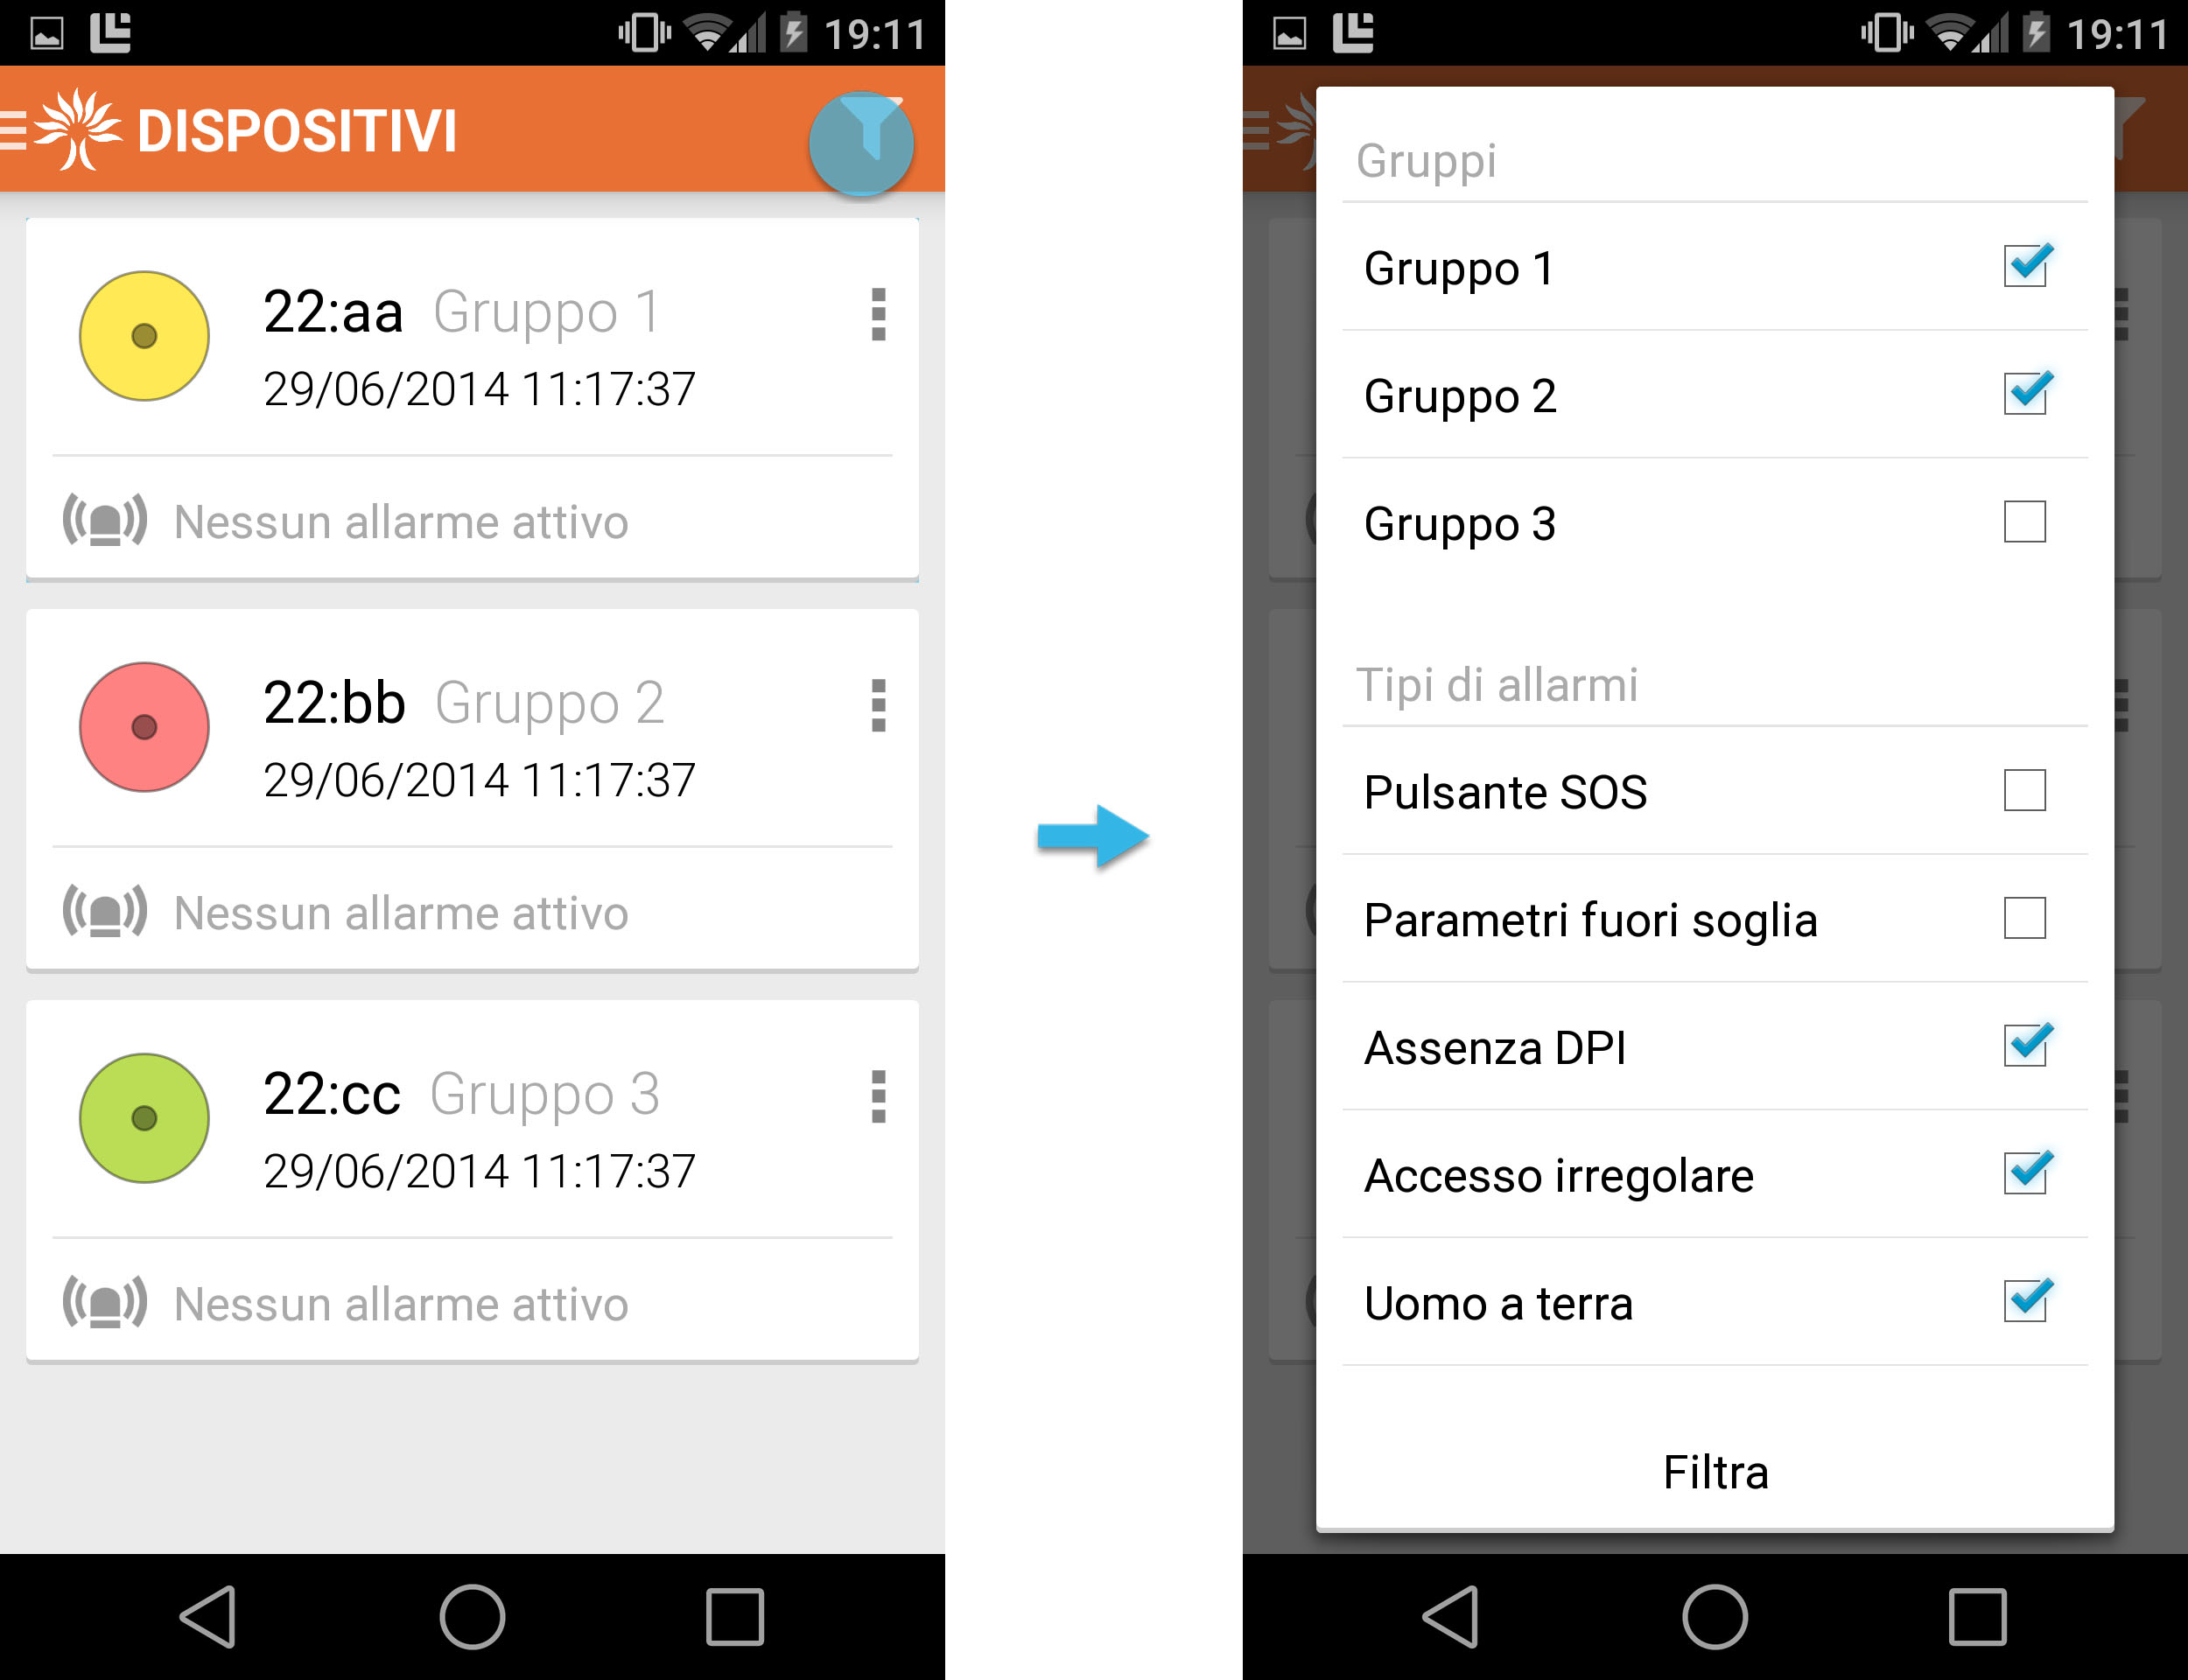
\includegraphics[width=0.8\textwidth]{phone_dispositivi_filter.jpg}}
		  \caption{Phone - Filter Dialog}
	\end{figure}

	\begin{figure}[h!]
		  \centering
		    \centering{%
		      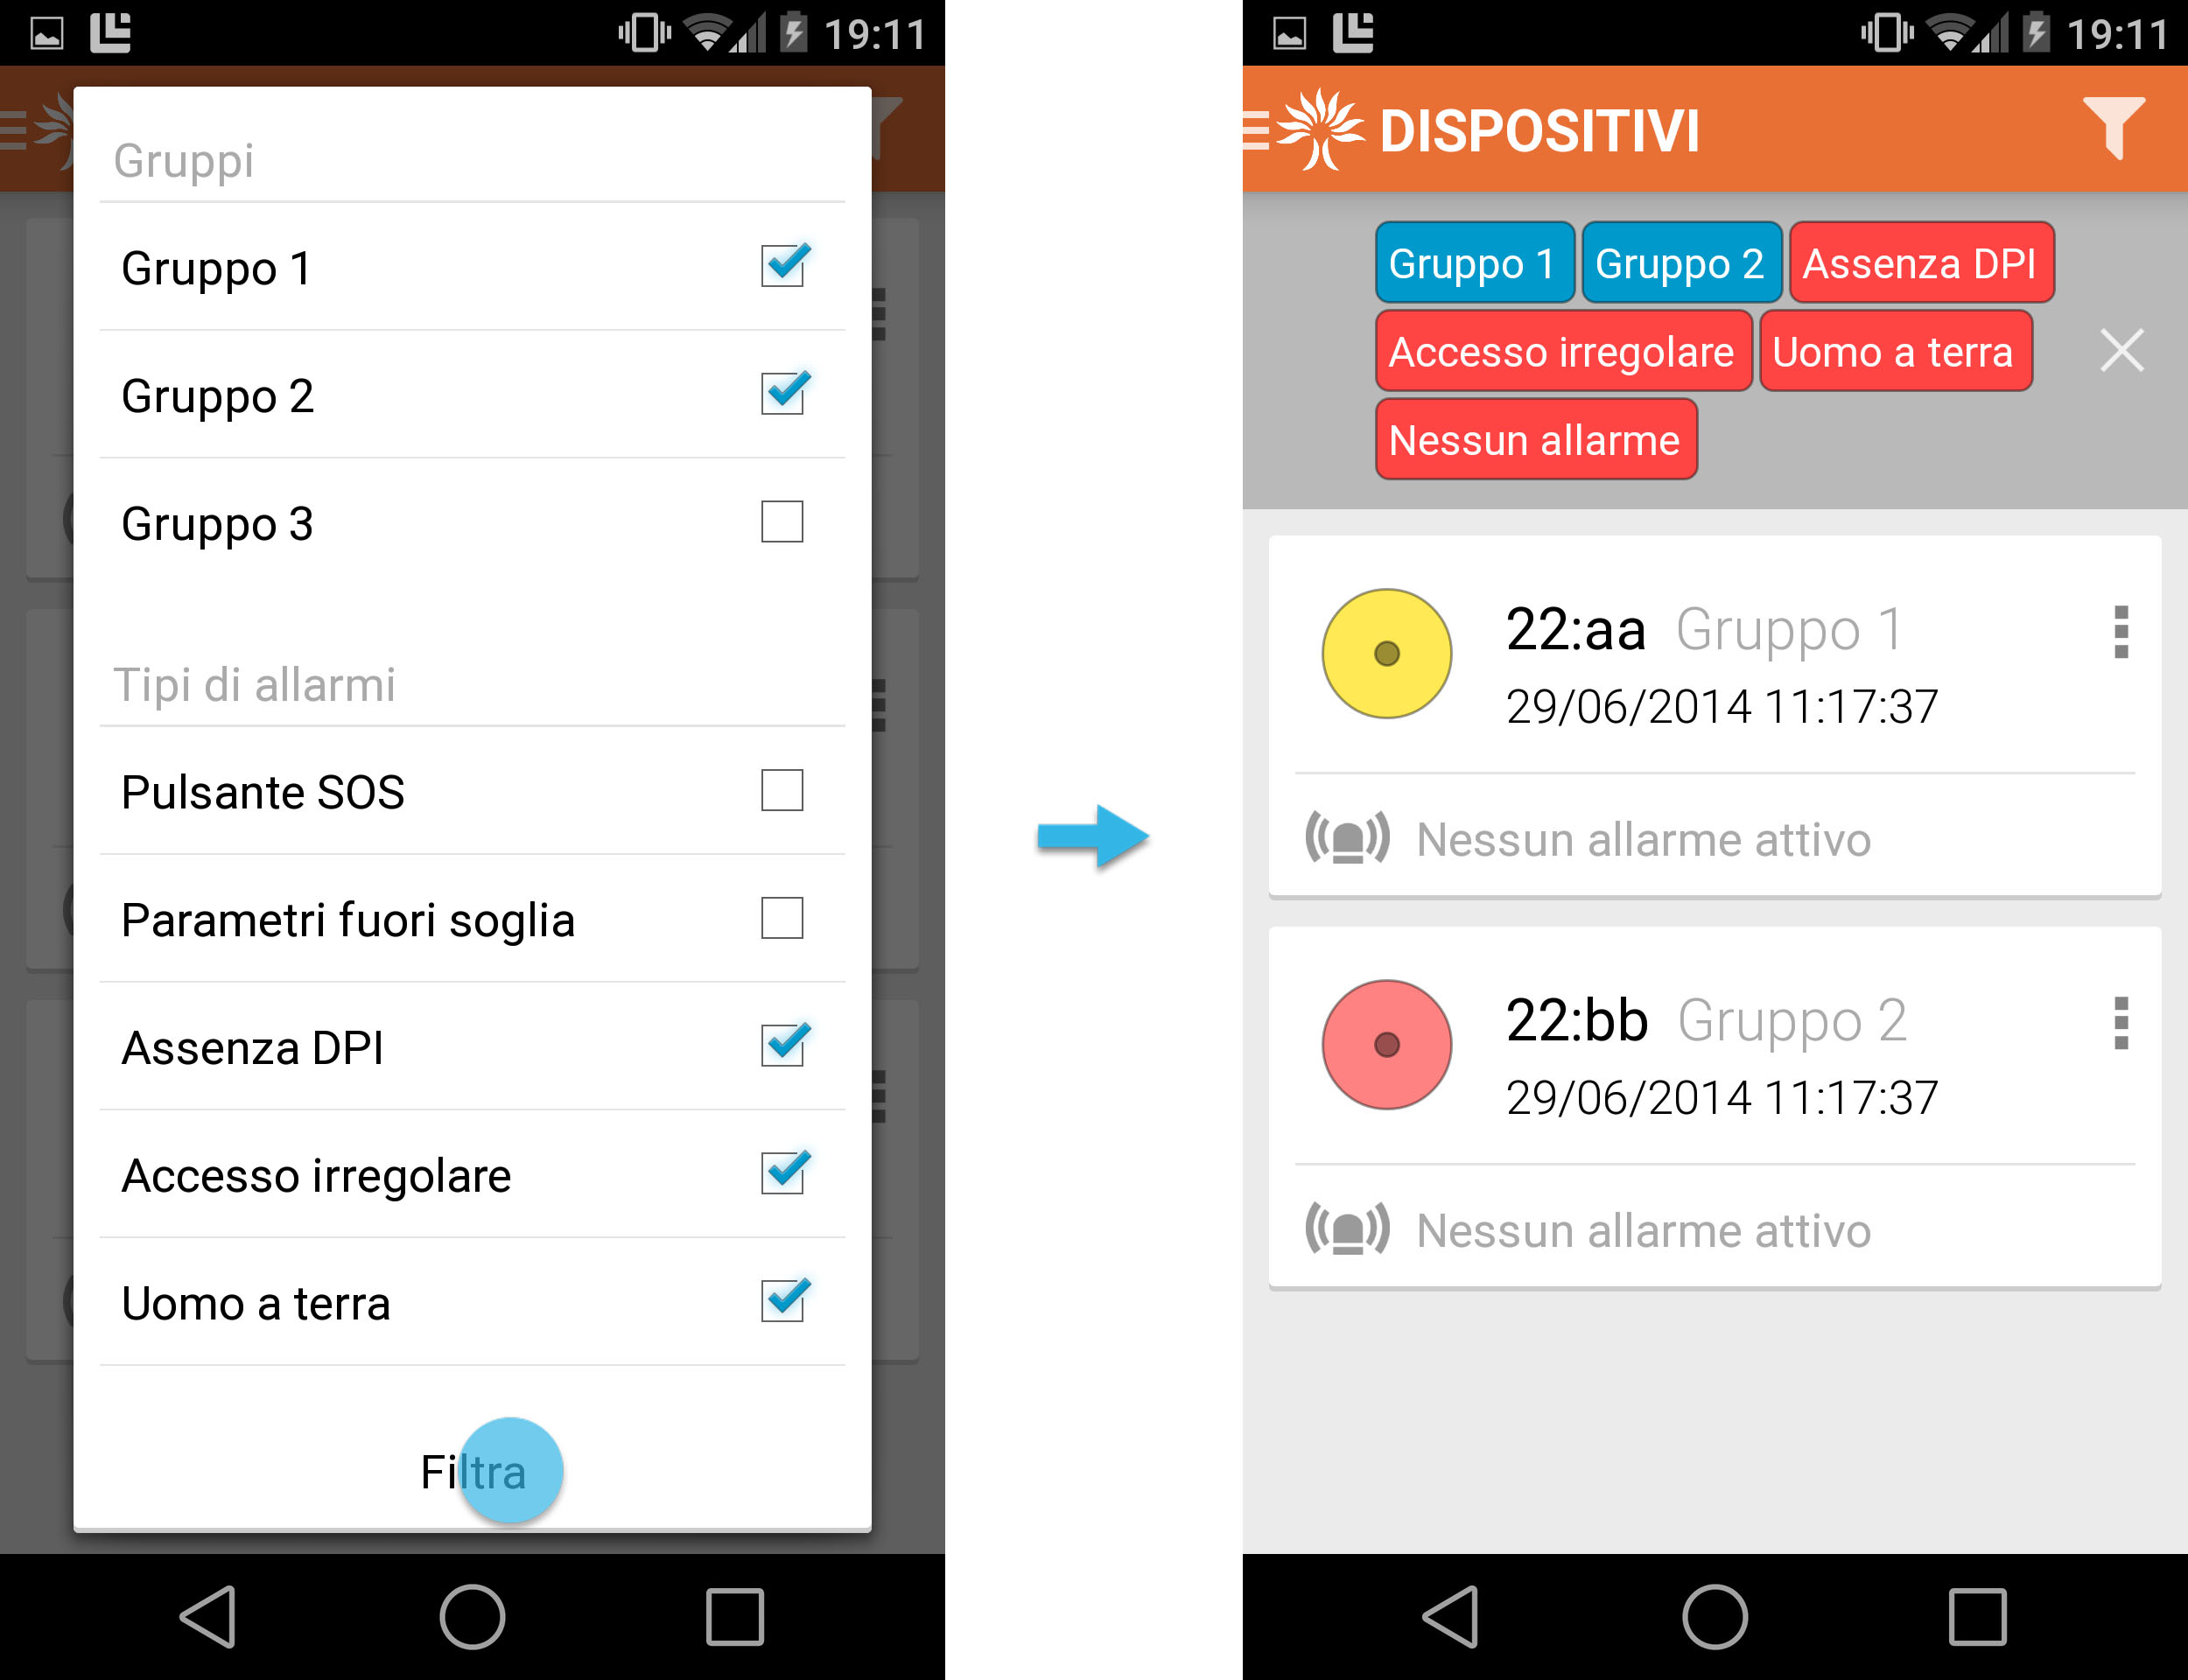
\includegraphics[width=0.8\textwidth]{phone_filter_dispositivi.jpg}}
		  \caption{Phone - Filtered devices}
	\end{figure}

	\begin{figure}[h!]
		  \centering
		    \centering{%
		      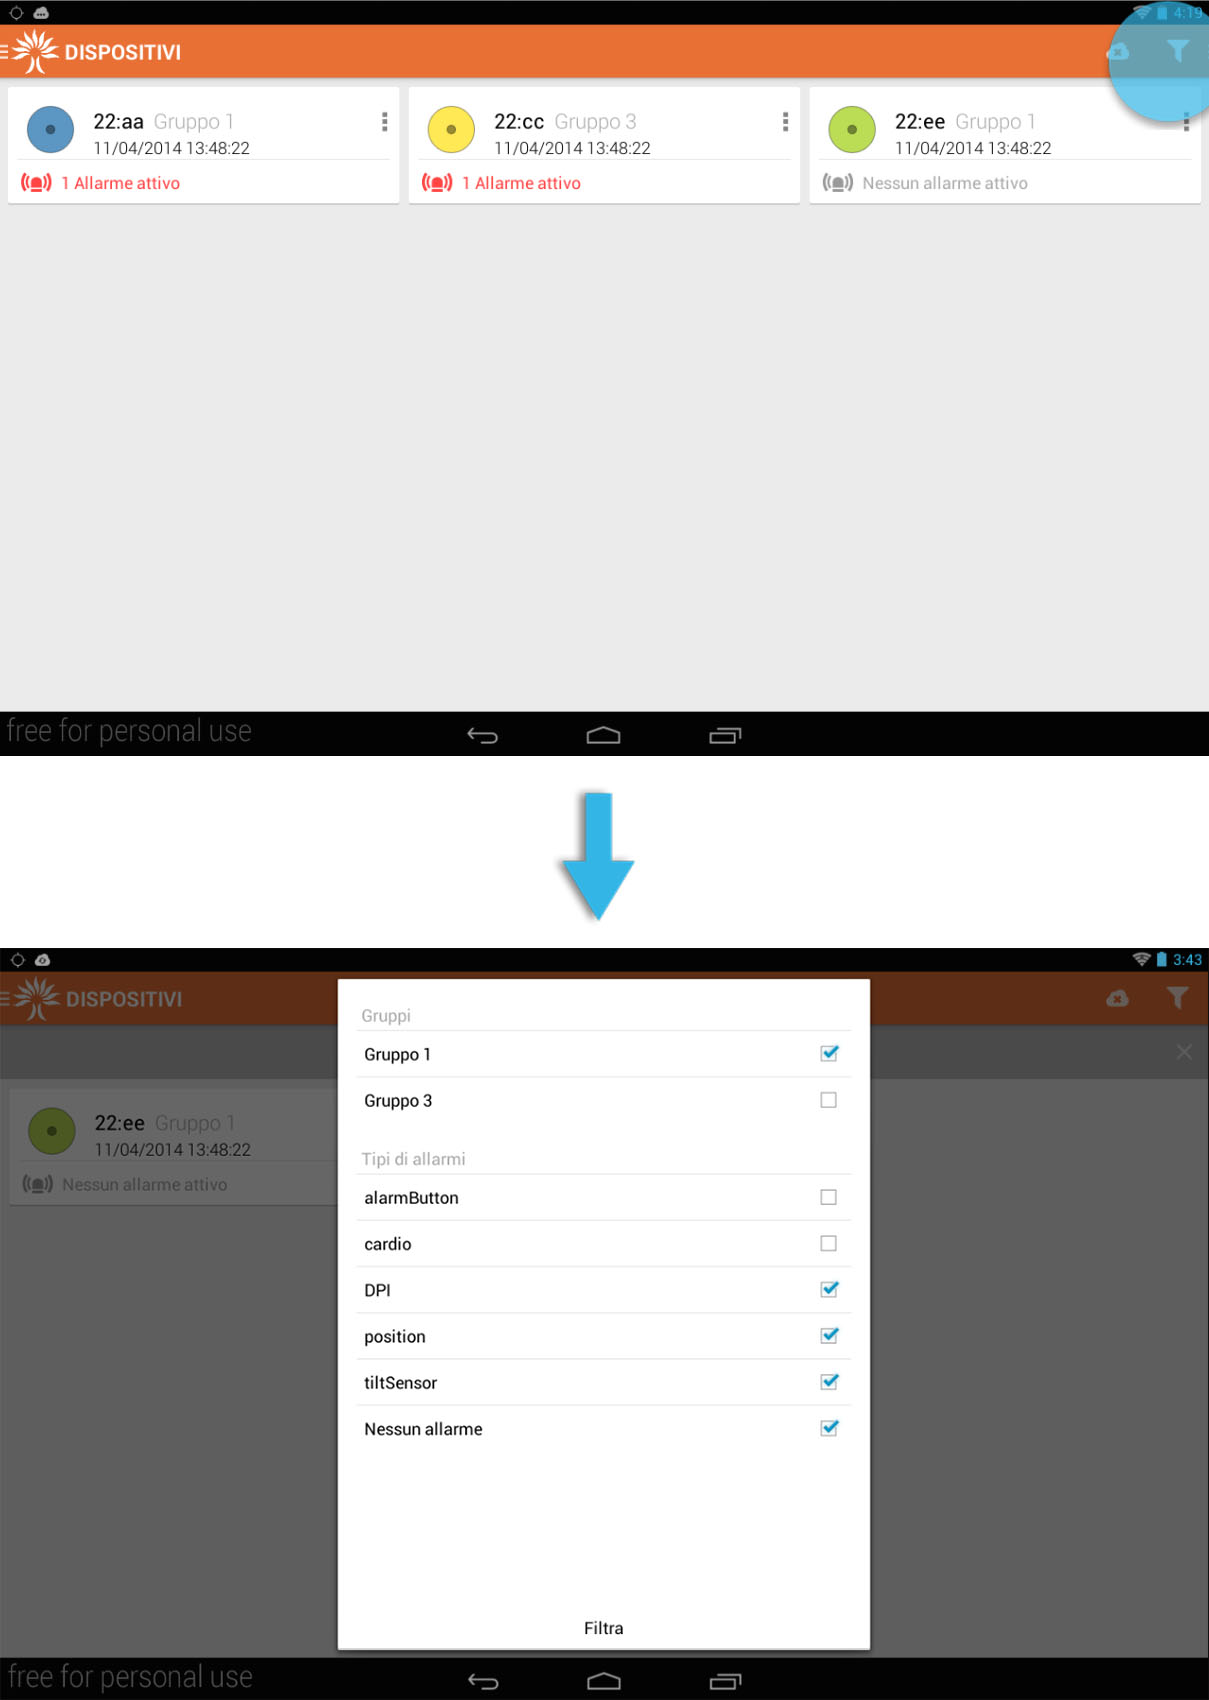
\includegraphics[width=1\textwidth]{tablet_dispositivi_filter.jpg}}
		  \caption{Tablet - Filter Dialog}
	\end{figure}

	\begin{figure}[h!]
		  \centering
		    \centering{%
		      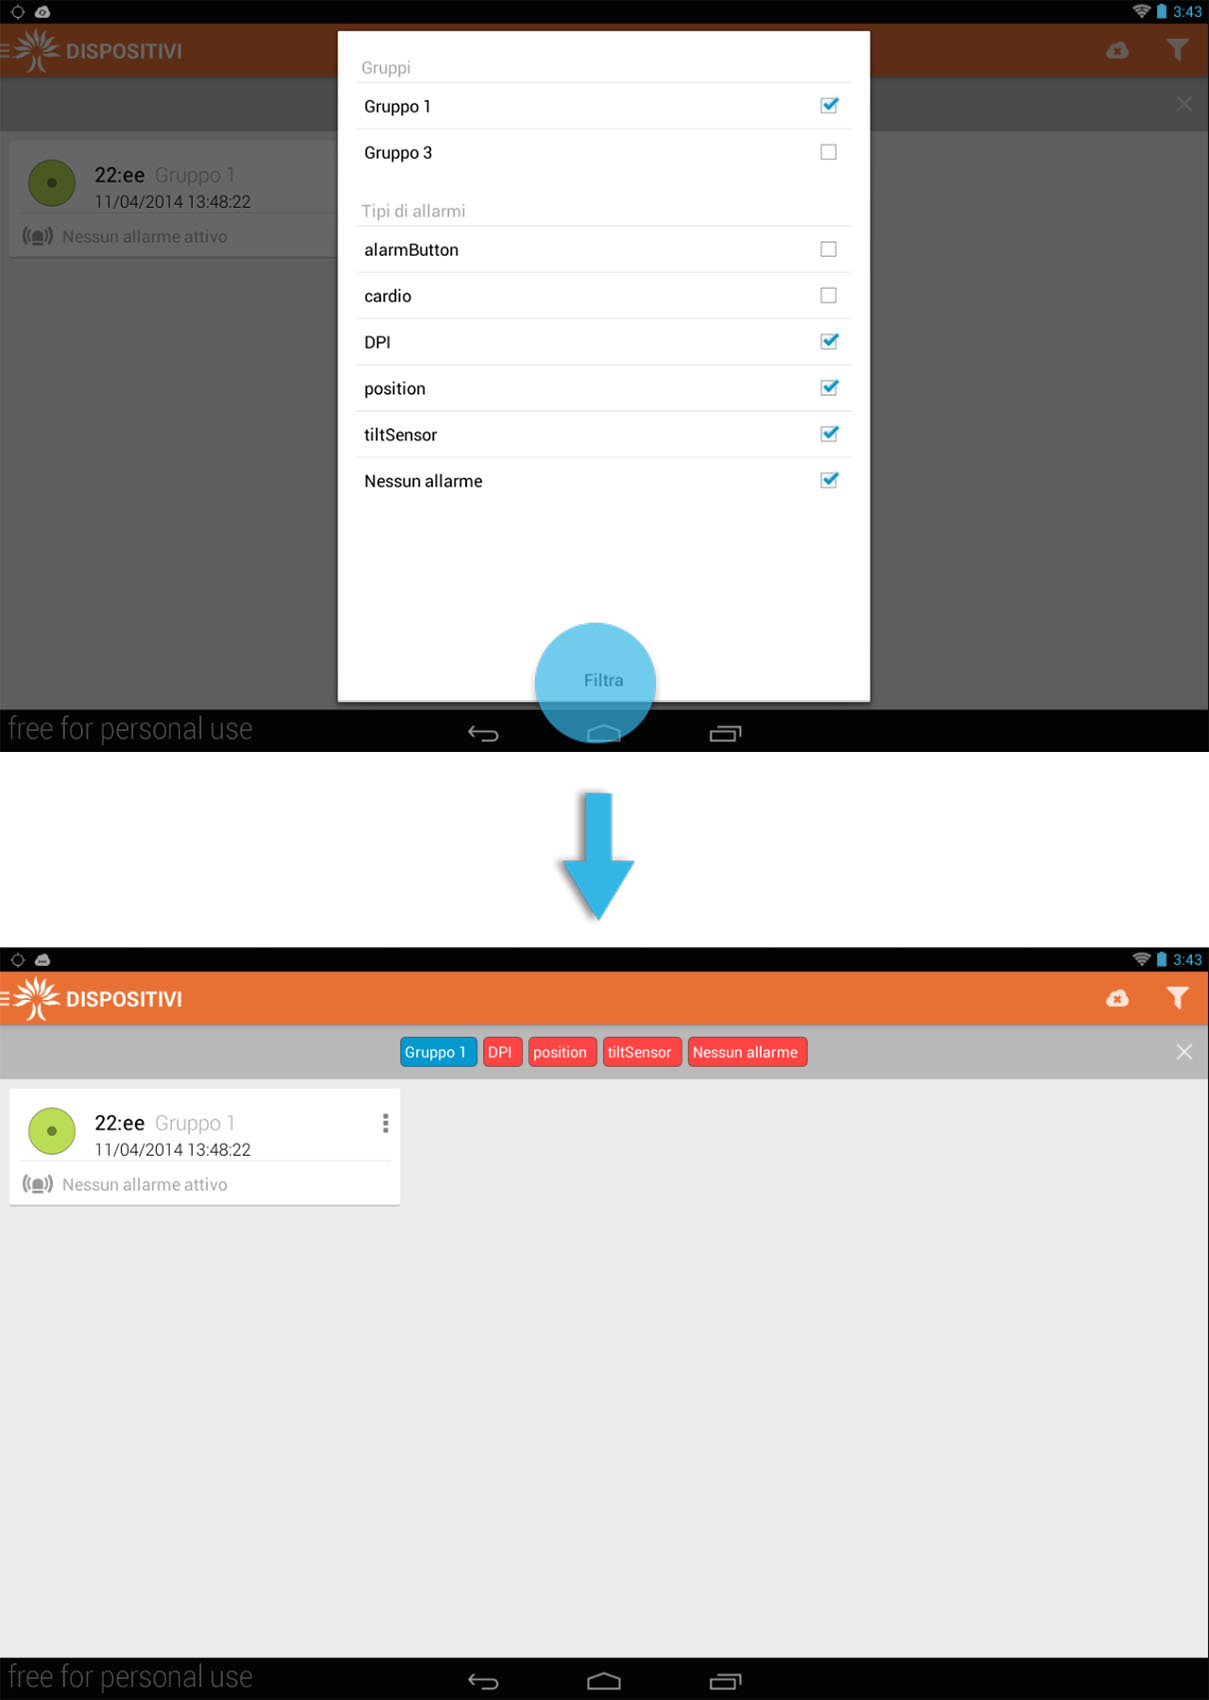
\includegraphics[width=1\textwidth]{tablet_filter_dispositivi.jpg}}
		  \caption{Tablet - Filtered devices}
	\end{figure}

